\documentclass{beamer} 
\usetheme{Warsaw}


\title{Inter-Packet Network Delays as a Time-Series Random Generator}
\author{Micah Thornton, Neha Joshi, Qiliang Zeng}
\date{\today}


\begin{document}

\begin{frame}
\maketitle{}
\end{frame}

\section{Introduction}

\begin{frame}
\tableofcontents{}
\end{frame}
\begin{frame}
\tableofcontents[hideallsubsections, 	currentsection]
\end{frame}


\subsection{Random Numbers \& Applications}

\begin{frame}
\frametitle{History of Random}

\begin{figure}
\vspace{- 1 em}
{\tiny \textsc{Figure 1: Ancient bone die used by Roman Empire circa 100-300 AD}}

\begin{center}
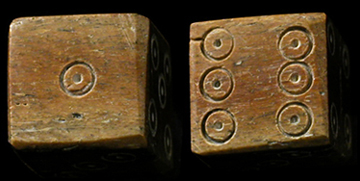
\includegraphics[scale=0.45]{images/ufdie.jpg} %http://www.ancientresource.com/lots/roman/roman_dice.html

\end{center}
\end{figure}

\vspace{- 1.5 em}
\begin{itemize}
		\item In ancient times, random values used for \textbf{gambling,  forecasting and fortune-telling}
		\item In modern times, they are used for \textbf{Security and Simulation}
		\item Process random iff all outcomes have equal odds of occurrence. (Shannon)
\end{itemize}
\end{frame}

\begin{frame}
\frametitle{Modern Applications of Random Values (1)}

\begin{figure}
\vspace{-1 em}
{\tiny \textsc{Figure 2: Example application of random values to public key cryptography}}\\
\vspace{0.5 em}
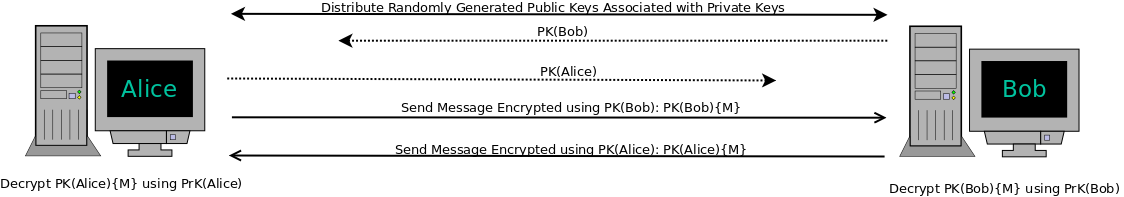
\includegraphics[scale = 0.25]{images/PKC.png}
\end{figure}


\begin{itemize}
	\item In cryptography:
	\begin{itemize}
		\item RSA: RNs are used to generate primes (No RNG specified)
		\item 3-DES: RNs used as key-bundle (Specific RNG ANSI x9.31)
		\item Blowfish: RN used a 52-bit key (No RNG specified)
		\item Twofish: RN used as up to 256-bit key (No RNG specified)
		\item AES: RNs used as key-IV-salt bundle (NIST specified RNG)
	\end{itemize}
	\item In science:
	\begin{itemize}
		\item Statistics: Taking random sample
		\item Analysis: Extraction of signal from noise
		\item Simulation: Providing a spectrum inputs
	\end{itemize}

\end{itemize}

\end{frame}

\begin{frame}
\frametitle{Modern Applications of Random Values (2)}

\begin{figure}
\vspace{-1.5 em}
{\tiny \textsc{Figure 3: Famous casino \& resort in Las Vegas}}\\
\vspace{0.5 em}
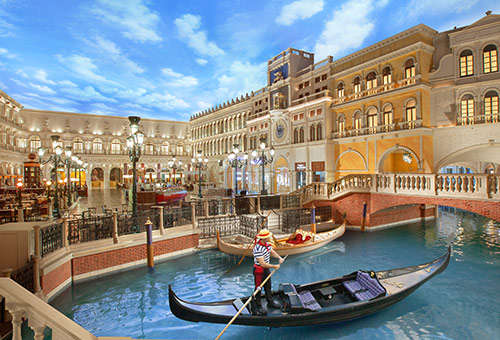
\includegraphics[scale = 0.25]{images/ven.jpeg}
\end{figure}
\vspace{-1 em}
\begin{itemize}
	\item In Gambling:
		\begin{itemize}
		\item Card Games: Poker, Black Jack, etc...
		\item Die Games: Craps
		\item Wheel Games: Roulette				
		\item Slot Machines:  `fair' results (usually biased)
	\end{itemize}
	\item In CSE 7344 Research Projects:
	\begin{itemize}
		\item Generation of Random IP addresses from a range (Mirai)
		\item Sending random packets (Domino)
	\end{itemize}
\end{itemize}
\end{frame}
\subsection{Random Generators}
\begin{frame}
\frametitle{Approaches to Random Generation}
\vspace{-1 em}

\begin{columns}
\begin{column}{0.5\textwidth}
{\tiny \textsc{Figure 4: Giuseppe Lodovico Lagrangia}}\\
\vspace{0.5 em}
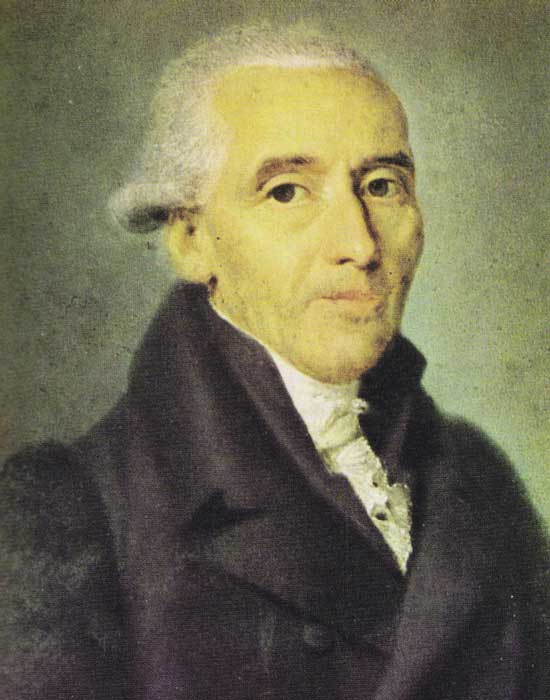
\includegraphics[scale = 0.25]{images/lag.jpg}
\end{column}
\begin{column}{0.65\textwidth}

\begin{itemize}
	\item Pseudo-Random Number Generators (PRNGs)
	\begin{itemize}
		\item Shift Registers (LFSR, NLFSR) - Golomb (1948)
		\item Linear Congruential Generators (LCG) - D. H. Lehmer (1949)
		\item Blum Blum Shub (BBS) - Blum,Blum, and Shub (1986) 
		\item Mersenne Twister (MT) - Matsumoto \& Nishimura (1997)
	\end{itemize}	
	\item True Random Number Generators (TRNGs)
	\begin{itemize}
		\item Atmospheric Noise (random.org)
		\item Radioactive Decay (hotbits.org)
	\end{itemize}
\end{itemize}

\end{column}
\end{columns}
\end{frame}

\begin{frame}
\frametitle{Entropy Extractors for TRNGs}
\begin{figure}
{\tiny \textsc{Figure 5: Example Entropy Extraction (The Hotbits way)}}\\
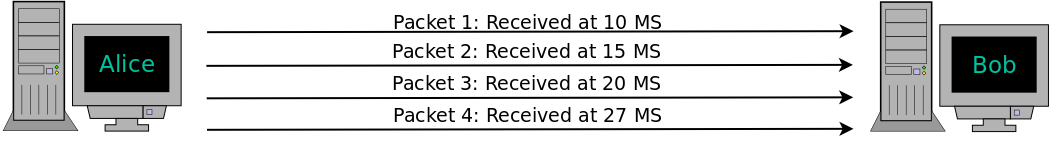
\includegraphics[scale = 0.25]{images/entext.png}
\end{figure}

\begin{columns}
\begin{column}{0.5\textwidth}
$$ T_1 = P_2 - P_1 = 15 - 10 = 5 $$
$$ T_2 = P_4 - P_3 = 27 - 20 = 7 $$
\end{column}
\begin{column}{0.5\textwidth}
if T1 $>$ T2: \\
    \hspace{2 em} record one\\
if T1 $<$ T2:\\
    \hspace{2 em} record zero\\
if T1 = T2: \\
    \hspace{2 em} record nothing

\end{column}
\end{columns}
\end{frame}
\section{Network Random Generator}
\begin{frame}
\tableofcontents[hideallsubsections, 	currentsection]
\end{frame}
\subsection{A Posteriori Extractor}
\begin{frame}
\frametitle{A Posteriori Extraction Method}
\begin{center}
Given $X$ such that $X=\{x_1,x_2,x_3,...,x_n\}$ \\
\end{center}
$$Q_2 = \{x \in X|P(X>x)=P(X<x)=0.5\}$$
$$R_\psi(x_i) = r_i = \begin{cases} 
      1 & x_i > Q_2 \\
      0 & x_i < Q_2
   \end{cases}$$
\begin{center}
Hence, the entropy is extracted into the binary value: $r_1r_2r_3r_4...r_n$ \\
\vspace{2 em}
\textit{Note: alternative measures of center can be used in the place of $Q_2$} \\
\textit{but only $Q_2$ maximizes the extracted entropy}
\end{center}

\end{frame}

\begin{frame}
\frametitle{A Posteriori Extractor for Inter-Packet Delays Example}
\vspace{- 2 em}
\begin{figure}
{\tiny \textsc{Figure 6: Example Entropy Extraction (A Posteriori method)}}\\
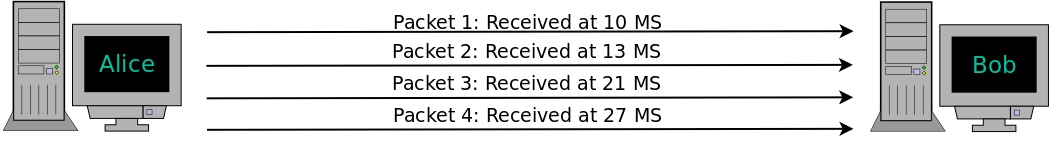
\includegraphics[scale = 0.25]{images/entext2.png}
\end{figure}

\begin{columns}
\begin{column}{0.5\textwidth}
$$ T_1 = P_2 - P_1 = 13 - 10 = 3 $$
$$ T_2 = P_3 - P_2 = 21 - 13 = 8 $$
$$ T_3 = P_4 - P_3 = 27 - 21 = 6 $$
$$ Q_2 = 6 $$
\end{column}
\vspace{ 1 em}
\begin{column}{0.5\textwidth}
for $T_i$: \\
\hspace{1 em}if $T_i > Q_2$: \\
    \hspace{2 em} record one\\
\hspace{1 em}else: \\
	\hspace{2 em} record zero
\end{column}
\end{columns}
\end{frame}

\begin{frame}
\frametitle{A Posteriori Maximizes Shannon's Entropy (1)}
{\tiny
\textbf{[PROOF:]}\\
\vspace{0.5 em}
Given a \textit{supposedly} random sample $$X = \{x_1 \in \mathbb{R},x_2\in \mathbb{R},x_3\in \mathbb{R},...,x_n\in \mathbb{R}\}$$We define the random variable $\alpha$ in terms of the median (or second quartile) of $X$ $$\alpha:\mathbb{R}\to\mathbb{B}$$ $$P(\alpha =  0) = p_0(\alpha) = \frac{\vert\{x\vert x<Q_2(X)\}\vert}{\vert X \vert} = \frac{1}{2} $$ $$P(\alpha =  1) = p_1(\alpha) = \frac{\vert\{x\vert x>Q_2(X)\}\vert}{\vert X \vert} = \frac{1}{2}$$The formula for the entropy of a string of Bernoulli trials (or a `bitstring') is given:$$H(p_0(b),p_1(b)) = -(p_0(b)\textrm{log}_2(p_0(b)) +p_1(b)\textrm{log}_2(p_1(b)))$$ We can maximize the Entropy function as so:$$\nabla H(p_0,p_1) = \Big(\frac{\partial H}{\partial p_0},\frac{\partial H}{\partial p_1}\Big) = \Big(-\frac{\textrm{ln}(p_0) + 1}{\textrm{ln}(2)},-\frac{\textrm{ln}(p_1) + 1}{\textrm{ln}(2)}\Big)$$Maximizing we find$$\frac{-\textrm{ln}(p_0) - 1}{\textrm{ln}(2)} = 0 \implies \textrm{ln}(p_0) = -1 \implies p_0 = \frac{1}{e}$$ $$\frac{-\textrm{ln}(p_1) - 1}{\textrm{ln}(2)} = 0 \implies \textrm{ln}(p_1) = -1 \implies p_1 = \frac{1}{e}$$}
\end{frame}
\begin{frame}
\frametitle{A Posteriori Maximizes Shannon's Entropy (2)}
{\tiny This seemingly odd result is because there is an \textit{inherent} dependence among these two values, expressed mathematically as $p_0 + p_1 = 1$, in our first maximization attempt, we neglected to account for the hard-restraint $p_0 +p_1 = 1$ In constraining the original optimization we have the following system: 
$$\frac{-\textrm{ln}(p_1) - 1}{\textrm{ln}(2)} = 0 = \frac{-\textrm{ln}(p_0) - 1}{\textrm{ln}(2)}$$
$$ p_1 = 1-p_0$$
$$ \frac{-\textrm{ln}(1-p_0) - 1}{\textrm{ln}(2)} = \frac{-\textrm{ln}(p_0) - 1}{\textrm{ln}(2)} \implies 1-p_0 = p_0$$$$ \implies p_0 = 0.5 \implies p_1 = 1 - 0.5 = 0.5$$Because $p_0(\alpha) = p_1(\alpha) = 0.5$ by definition, we have maximized the entropy function for the constraint $p_1 + p_0 = 1$.\hfill  $\qed$}
\end{frame}

\subsection{Inter-Packet Timings \& Data Production}
\begin{frame}
\frametitle{Experimental Set-Up}
\begin{itemize}
\item Inter-Packet Timings: time differences between packet arrivals
\item Arrival times (in $\mu s$) captured by Wireshark \& TCPdump
\item Five machines used: 
\end{itemize}

\begin{table}
\begin{tabular}{|l|l|l|l|l|}
\hline
\textbf{Machine} & \textbf{OS} &\textbf{CPUs} &\textbf{RAM} &\textbf{Speed} \\
\hline
1 & Windows 10 & 2 & 8 Gb & 2.35 GHz \\ 
\hline 
2 & MacOS 10.12 & 2 & 8 Gb & 2.6 GHz \\
\hline 
3 & Ubuntu 16.10 & 8 & 16 Gb &  2.6 GHz \\ 
\hline 
4 & Ubuntu 17.04 & 8 & 16 Gb & 2.8 GHz \\
\hline 
5 & Ubuntu 17.04 & 8 & 32 Gb & 3.2 GHz \\
\hline
\end{tabular}
\end{table}
\end{frame}
\section{Results}
\begin{frame}
\tableofcontents[hideallsubsections, 	currentsection]
\end{frame}

\subsection{ENT results}
\begin{frame}
\frametitle{Initial Packet Capture Timings}

\begin{figure}
{\tiny \textsc{Figure 7: Initial Packet Captures (Wireshark)}}\\
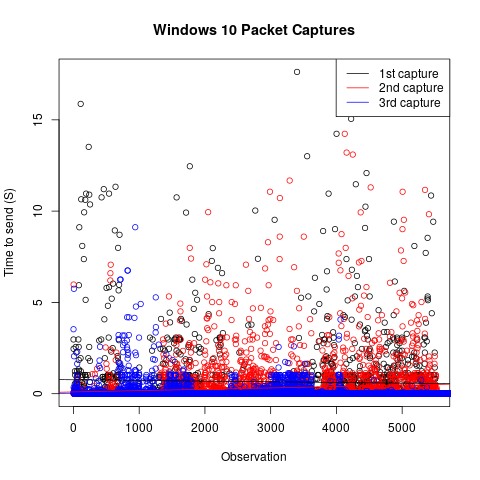
\includegraphics[scale = 0.22]{images/Neha2.png}
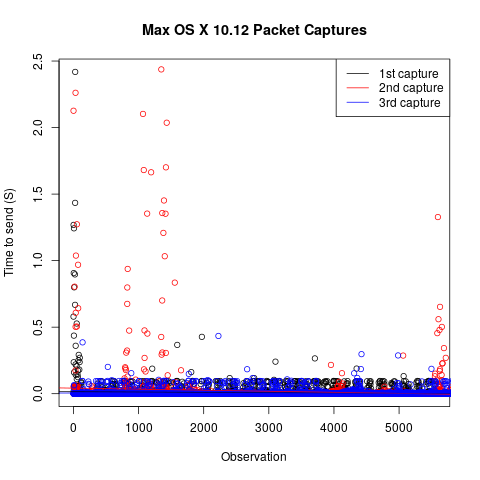
\includegraphics[scale = 0.22]{images/Zeng2.png}
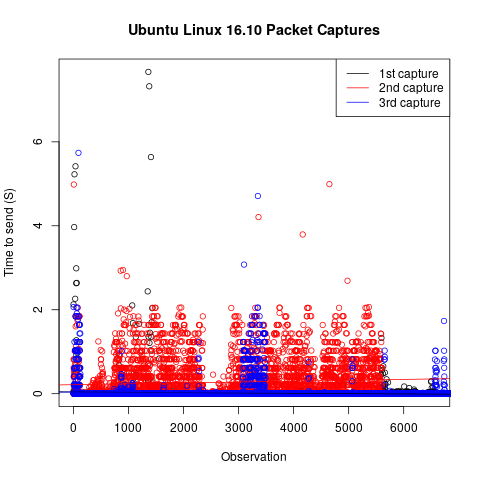
\includegraphics[scale = 0.22]{images/Micah2.png}
\end{figure}


\begin{itemize}
	\item 3 Captures done on machines 1-3  $\approx$ 5000 packets ea.
	\item Significant fraction of data is below 100 ms
	\item Note: Scales are different (Mac OSX streaming during cap.)
\end{itemize}

\end{frame}

\begin{frame}
\frametitle{ENT results}
\begin{figure}
{\tiny \textsc{Figure 8: Fourmilabs ENT results}}\\
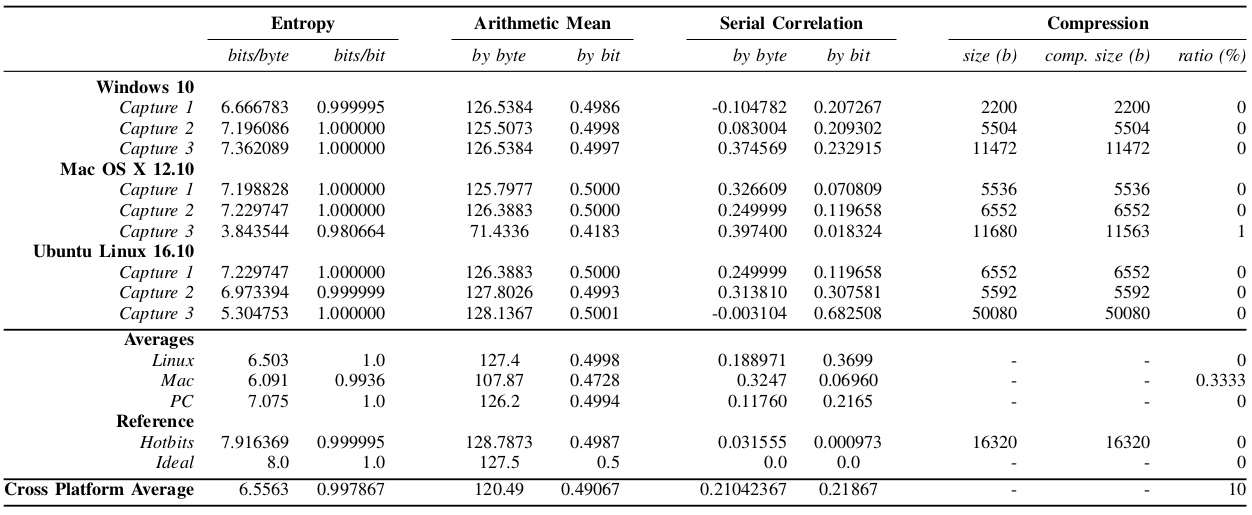
\includegraphics[scale = 0.33]{images/pet.png}
\end{figure}
\end{frame}

\subsection{Hashing Random Values}
\begin{frame}
\frametitle{Before and After on an Idle Network}
\begin{columns}
\begin{column}{0.5\textwidth}
\begin{figure}
{\tiny \textsc{Figure 9: Idle Before Hashing}}\\
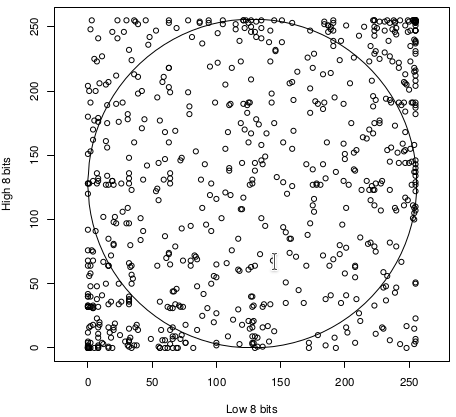
\includegraphics[scale = 0.43]{images/ibh.png}
\end{figure}
\end{column}
\begin{column}{0.5\textwidth}
\begin{figure}
{\tiny \textsc{Figure 10: Idle After Hashing}}\\
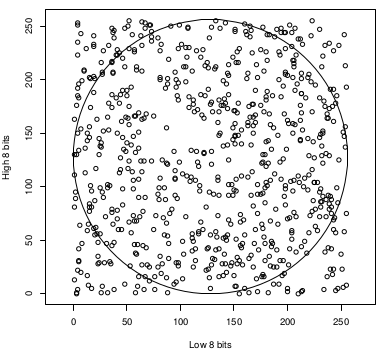
\includegraphics[scale = 0.5]{images/iah.png}
\end{figure}
\end{column}
\end{columns}
\end{frame}

\begin{frame}
\frametitle{Before and After on Busy Network}
\begin{columns}
\begin{column}{0.5\textwidth}
\begin{figure}
{\tiny \textsc{Figure 11: Busy Before Hashing}}\\
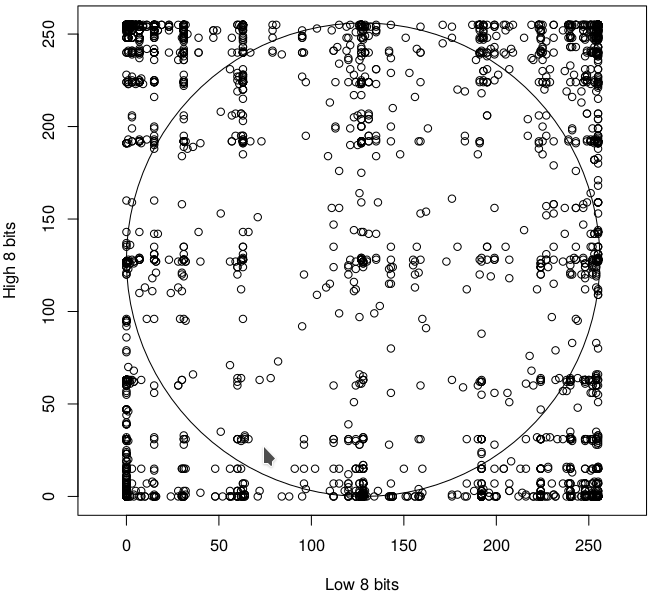
\includegraphics[scale = 0.32]{images/bbh.png}
\end{figure}
\end{column}
\begin{column}{0.5\textwidth}
\begin{figure}
{\tiny \textsc{Figure 12: Busy After Hashing}}\\
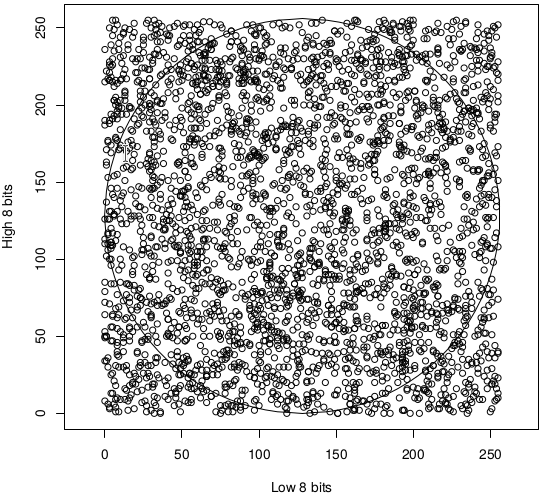
\includegraphics[scale = 0.39]{images/bah.png}
\end{figure}
\end{column}
\end{columns}
\end{frame}
\section{Conclusions}
\begin{frame}
\tableofcontents[hideallsubsections, 	currentsection]
\end{frame}

\subsection{Pros \& Applicability}
\begin{frame}
\frametitle{Pros \& Applicability}
\begin{itemize}
	\item Most modern-day PCs have network cards
	\item Could offer extra source of entropy
	\item Mixing with other sources is possible
	\item Two or more sources is shown to have better properties
	\item Could also be injected into dev/random in Linux
\end{itemize}
\begin{figure}

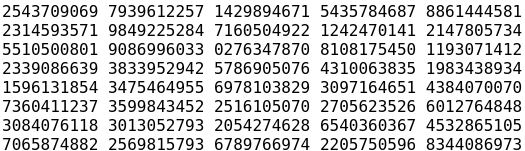
\includegraphics[scale = 0.5]{images/pi.png} \\
{\tiny \textsc{Figure 13: Random Numbers?}}
\end{figure}
\end{frame}
\subsection{Potential Improvement \& Future Work}

\begin{frame}
\frametitle{Potential Improvement \& Future Work}

\begin{figure}

\includegraphics[scale=0.5]{images/nist.png}
\end{figure}
\begin{itemize}
	\item We have accumulated $\approx$ 8 Mb of random data
	\item We have preliminary NIST STS results and Dieharder Results
	\item Test strategy on different networks and devices
	\item Attempt method with different time series
	\item Intend to use Hummingbird 2 python script written during this project, in place of hash
	\item Suggestions? 
\end{itemize}
\end{frame}

\begin{frame}
\frametitle{Thankyou for your Attention: Questions?}

\begin{center}
{\tiny \textsc{Figure 15: Monkey on Typewriter}}\\
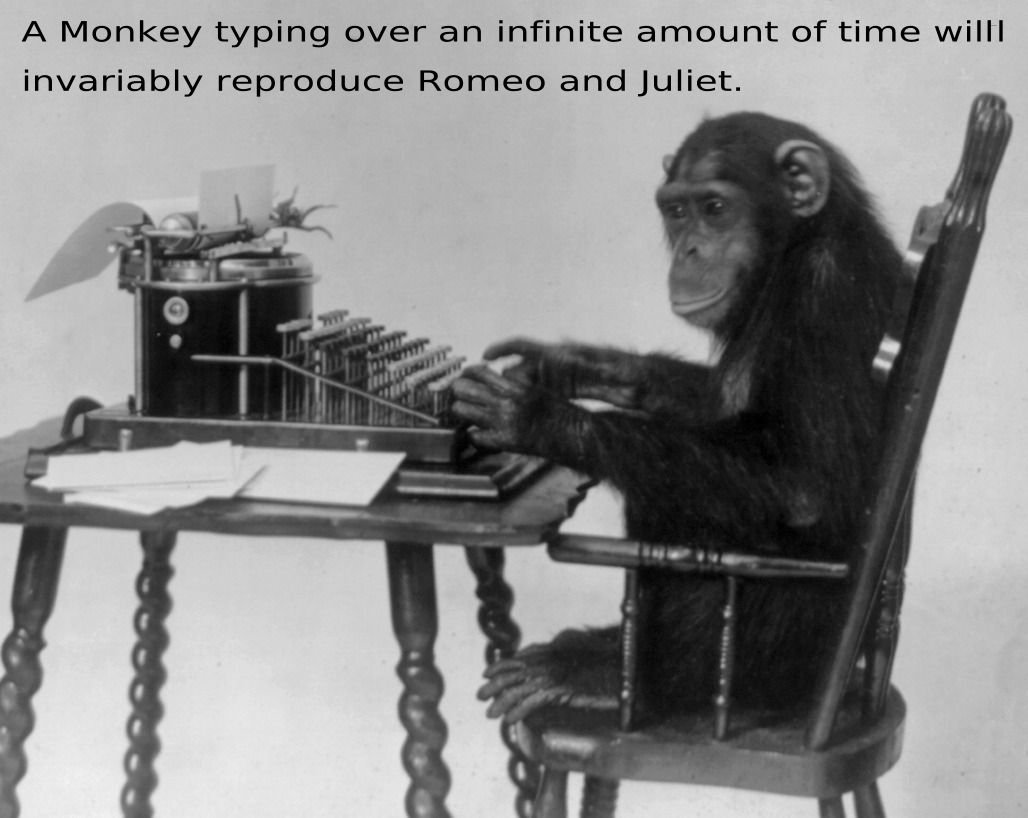
\includegraphics[scale = 0.35]{images/crj3.jpg}
\end{center}
\end{frame}

\begin{frame}
\frametitle{References}
\end{frame}


\end{document}